\documentclass[a4paper,11pt,twoside]{scrartcl}
\usepackage[T1]{fontenc}
\usepackage[utf8]{inputenc}
\usepackage{ngerman, eucal, mathrsfs, amsfonts, bbm, amsmath, amssymb, stmaryrd, array, xcolor,graphicx, float, wrapfig}
\usepackage{epstopdf}
\usepackage{listings}
\usepackage[official]{eurosym}
\DeclareUnicodeCharacter{20AC}{\EUR{}}


\definecolor{middlegray}{rgb}{0.5,0.5,0.5}
\definecolor{lightgray}{rgb}{0.8,0.8,0.8}
\definecolor{orange}{rgb}{0.8,0.3,0.3}
\definecolor{yac}{rgb}{0.6,0.6,0.1}
\definecolor{green}{rgb}{0,.5,0}

\lstdefinestyle{c}{
	keywordstyle=\bfseries\ttfamily\color{blue},
	stringstyle=\color{orange}\ttfamily,
	commentstyle=\color{green}\ttfamily,
	emph={@Override, while, forall, if}, 
	emphstyle=\color{green}\texttt,
	emph={[2]List, Queue},
	emphstyle={[2]\color{yac}\texttt},
}
\lstset{
	basicstyle=\ttfamily,
	showstringspaces=false,
	flexiblecolumns=true,
	tabsize=2,
	numbers=left,
	numberstyle=\tiny,
	numberblanklines=false,
	stepnumber=1,
	numbersep=10pt,
	xleftmargin=15pt,
	breaklines=true,
	inputencoding=utf8
}

\lstdefinestyle{java}{
	language = java,
	emph={@Override}, 
	emphstyle=\color{teal}\texttt,
	emph={[2]Node,T,Comparable,AbstractNode,System, Thread,Random, Tree, Integer, Math, String, InterruptedException, Map, Entry, Point, TreeMap, PrintWriter, Scanner, FileReader, FileInputStream, FileNotFoundException, InputStreamReader, UnsupportedEncodingException, DecimalFormat, ArrayList, HashSet, LinkedList, IOException, HashMap, MapTest, MyHashMap, Puzzle, MyQueue, StringBuilder, NoSuchElementException, List, Queue, Vector, Tuple,Search, IllegalArgumentException, UnionFind, AbstractUnionFind, SpanningTree, Collections, WeightedEdge},
	emphstyle={[2]\color{yac}\texttt},
	texcl=true,
	keywordstyle=\color{blue}\ttfamily,
	stringstyle=\color{red}\ttfamily,
	commentstyle=\color{green}\ttfamily
}

\lstset{literate=
	{á}{{\'a}}1 {é}{{\'e}}1 {í}{{\'i}}1 {ó}{{\'o}}1 {ú}{{\'u}}1
	{Á}{{\'A}}1 {É}{{\'E}}1 {Í}{{\'I}}1 {Ó}{{\'O}}1 {Ú}{{\'U}}1
	{à}{{\`a}}1 {è}{{\`e}}1 {ì}{{\`i}}1 {ò}{{\`o}}1 {ù}{{\`u}}1
	{À}{{\`A}}1 {È}{{\'E}}1 {Ì}{{\`I}}1 {Ò}{{\`O}}1 {Ù}{{\`U}}1
	{ä}{{\"a}}1 {ë}{{\"e}}1 {ï}{{\"i}}1 {ö}{{\"o}}1 {ü}{{\"u}}1
	{Ä}{{\"A}}1 {Ë}{{\"E}}1 {Ï}{{\"I}}1 {Ö}{{\"O}}1 {Ü}{{\"U}}1
	{â}{{\^a}}1 {ê}{{\^e}}1 {î}{{\^i}}1 {ô}{{\^o}}1 {û}{{\^u}}1
	{Â}{{\^A}}1 {Ê}{{\^E}}1 {Î}{{\^I}}1 {Ô}{{\^O}}1 {Û}{{\^U}}1
	{œ}{{\oe}}1 {Œ}{{\OE}}1 {æ}{{\ae}}1 {Æ}{{\AE}}1 {ß}{{\ss}}1
	{ű}{{\H{u}}}1 {Ű}{{\H{U}}}1 {ő}{{\H{o}}}1 {Ő}{{\H{O}}}1
	{ç}{{\c c}}1 {Ç}{{\c C}}1 {ø}{{\o}}1 {å}{{\r a}}1 {Å}{{\r A}}1
	{€}{{\EUR}}1 {£}{{\pounds}}1
}
\usepackage{geometry}
\geometry{left=25mm, right=15mm, bottom=25mm}
\setlength{\parindent}{0em} 
\setlength{\headheight}{0em} 

\title{Datenstrukturen und effiziente Algorithmen\\ Blatt 11}
\author{Markus Vieth, David Klopp, Christian Stricker}
\date{\today}



\begin{document}

\maketitle
\cleardoublepage
\pagestyle{myheadings}
\markboth{Markus Vieth,  David Klopp, Christian Stricker}{Markus Vieth, David Klopp, Christian Stricker}

\section*{Aufgabe 1}
\subsection*{Python-Code}
\lstinputlisting[style=python,basicstyle=\small\ttfamily]{Code/wordCount.py}

Die Anzahl der Buchstaben beträgt 2252.



\section*{Aufgabe 2}

\subsection*{Pseudo-Code}
\lstinputlisting[style=c,basicstyle=\small\ttfamily]{Code/linearList.c}

\subsection*{Beschreibung}
Füge drei Knoten in den Fibonacci-Heap ein. Der erste Knoten ist hierbei um 1 größer, der zweite um 1 kleiner und der dritte um 2 kleiner als das aktuelle Minimum. Lösche nun den Minimumknoten, aktualisiere ihn und setzte den Wert des Größten Kindes des neuen Minimumknotens auf das aktuelle Minimum -2. Es ergibt sich somit ein neues Minimum, das in die Wurzelliste aufgenommen wird. Dieses wird nun abschließend gelöscht. In jedem Schritt wird so also genau ein Knoten in den Heap eingefügt. Es ergibt sich somit eine vertikale Liste.

%\subsection*{Beispiel}

\pagebreak

\section*{Aufgabe 3}

\subsection*{a)}

\subsubsection*{Hilfsmethode}
\begin{lstlisting}[style=c,basicstyle=\small\ttfamily]
int left(int i) {
	return 2i+1;
}

int right(int i) {
	return  2i+2;
}

int parent(int i) {
	return floor((i-1)/2);
}

// Heap-Eigenschaft herstellen
void heapify(Array b, int i) {
	// kleinstes Element des Asts finden 
	int min = i
	if (left(i) < b.size && b[left(i)].key < b[min].key)
		min = left(i)
	if (right(i) < b.size && b[right(i)].key < b[min].key)
		min = right(i)
		
	// wenn ein kleines Element existiert dann stelle die Heap-Eigenschaft her
	if (min != i) {
		b.swap(i, min)
		// verfahre kaskadenartig weiter
		heapify(b, min)
	}
}

\end{lstlisting}

\subsubsection*{decreaseKey}
\begin{lstlisting}[style=c,basicstyle=\small\ttfamily]
bool decrease(Array b, int i, newKey) {
	// neuer Schlüssel muss kleiner sein als alter
	if (newKey > b[i].key)
		return false;
	
	// Schlüssel setzten
 	b[i].key = newKey;
	
	// Heap-Eigenschaft herstellen
	while (i > 0 && b[i].key < b[parent(i)].key)) {
    		b.swap(i, parent(i));
    		i = parent(i);
	}
	return true;
}
\end{lstlisting}


\pagebreak


\subsubsection*{deleteMin}
\begin{lstlisting}[style=c,basicstyle=\small\ttfamily]
int deleteMin(Array b) {
	if (i<b.size)
		return -1; // Index out of bounds
	min = b[0];
	b.swap(i, -1); // sei -1 der Index des letzten Elements
	b.size -= 1 // verringere die Array Größe um 1

	// Heap-Eigenschaft herstellen
	if ((b.size > 0)
		heapify(b, i)
	return min;	
}
\end{lstlisting}


\subsubsection*{insert}
\begin{lstlisting}[style=c,basicstyle=\small\ttfamily]
void insert(Array b, newKey) {
	int i = b.size
	b.size += 1;
	// setzte b auf den höchst möglichen Wert
	b.key = MAX_INT 
	// Update den Wert und die Heap-Eigenschaft mit decrease
	decrease(b, i, newKey)
}
\end{lstlisting}


\subsection*{b)}
Die Laufzeit für die decreaseKey Operation beträgt $O(Baumtiefe) = O(\log(n))$. Unter der Annahme, dass das Resizen des Arrays in konstanter Zeit realisiert werden kann, beträgt somit die Laufzeit für insert ebenfalls $O(\log(n))$. Ausschlaggebend für die deleteMin Operation ist die heapify Methode, da sich der Rest der Implementierung in konstanter Zeit realisieren lässt. Die Laufzeit für heapify und somit auch für deleteMin beträgt ebenfalls $O(Baumtiefe) = O(\log(n))$.

\subsection*{c)}
Füge alle Elemente unsortiert in ein Array ein. Laufzeit: $O(1)$.\\
Wende nun Radix-Sort auf das Array an, um es zu sortieren. Laufzeit: $O(n)$. (Siehe hierzu VL 11)\\
Die Heap-Eigenschaft ist nun für alle Knoten erfüllt.

\section*{Zusatz 1}
\subsection*{a)}
\paragraph{Behauptung}
$(E,M) = (\{ a,b,c,d \}, \{ \emptyset,\{ a \},\{ b \},\{ c \}\{ d \}\}  )$ ist ein Matroid.
\paragraph{Beweis}
\subparagraph{zu zeigen: Nicht-Leerheit}
\[ \emptyset\in M=\{  \emptyset,\{ a \},\{ b \},\{ c \}\{ d \}\} \} \]
\subparagraph{zu zeigen: Vererbung}
Die Teilmengen einer einelementigen Menge sind die Menge selbst und die leere Menge. Somit ist offensichtlich, dass auch diese Bedingung erfüllt ist.
\subparagraph{zu zeigen: Austausch}
Sei $X$ eine der einelementigen Mengen aus $M$. Das einzige Element mit geringerer Kardinalität ist die leere Menge.
\[\Rightarrow \exists x\in X\setminus\emptyset=X | \{ x \}\cup\emptyset=X\in M \]
$\Rightarrow$ $(E,M)$ ist ein Matroid.
\subsection*{b)}
\paragraph{Nich-Leerheit}
$M$ muss die leere Menge enthalten $\Rightarrow$ $M':=\{ \emptyset,\{a,b \},\{ c,d \}\}\subseteq M$.
\paragraph{Vererbung}
Sei $\mathcal{P}(X)$ die Potenzmenge der Menge $X$\\
\[ M'\cup\mathcal{P}(\emptyset)\cup\mathcal{P}(\{a,b\})\cup\mathcal{P}(\{c,d\}) = \{ \emptyset,\{a,b \},\{ c,d \},\{ a \},\{ b \},\{ c \},\{ d \} \}=:M''\subseteq M \]
\paragraph{Austausch}
Wie in Teilaufgabe a) erklärt, muss die leere Menge nicht weiter betrachtet werden, da mit dieser lediglich die einelementigen Mengen erzeugt werden können.
\begin{description}
	\item[$A=\{v\},B=\{v,w\}$ mit $v,w\in E$] $B\setminus A = \{w\}, \{w\}\cup A = \{v,w\}$
	\item[$A=\{a\},B=\{c,d\}$] $B\setminus A = \{c,d\} \Rightarrow \{c\}\cup\{a\}=\{a,c\}\in M \veebar \{d\}\cup\{a\}=\{a,d\}\in M$
	\item[$A=\{b\},B=\{c,d\}$] $B\setminus A = \{c,d\} \Rightarrow \{c\}\cup\{b\}=\{b,c\}\in M \veebar \{d\}\cup\{b\}=\{b,d\}\in M$
	\item[$A=\{c\},B=\{a,b\}$] $B\setminus A = \{a,b\} \Rightarrow \{a\}\cup\{c\}=\{a,c\}\in M \veebar \{b\}\cup\{c\}=\{b,c\}\in M$
	\item[$A=\{d\},B=\{a,b\}$] $B\setminus A = \{a,b\} \Rightarrow \{a\}\cup\{d\}=\{a,d\}\in M \veebar \{b\}\cup\{d\}=\{b,d\}\in M$
\end{description}
\[\Rightarrow M=\{ \emptyset,\{a,b \},\{ c,d \},\{ a \},\{ b \},\{ c \},\{ d \},\{a,c\},\{b,d\} \}\veebar M=\{ \emptyset,\{a,b \},\{ c,d \},\{ a \},\{ b \},\{ c \},\{ d \},\{a,d\},\{b,c\} \}\]
$\Rightarrow(E,M)$ ist der kleinste Matroid, welcher den Anforderungen entspricht.
\begin{flushright}
	q.e.d.
\end{flushright}
\pagebreak
\section*{Zusatz 2}
\subsection*{a)}
\begin{figure}[H]
\centering
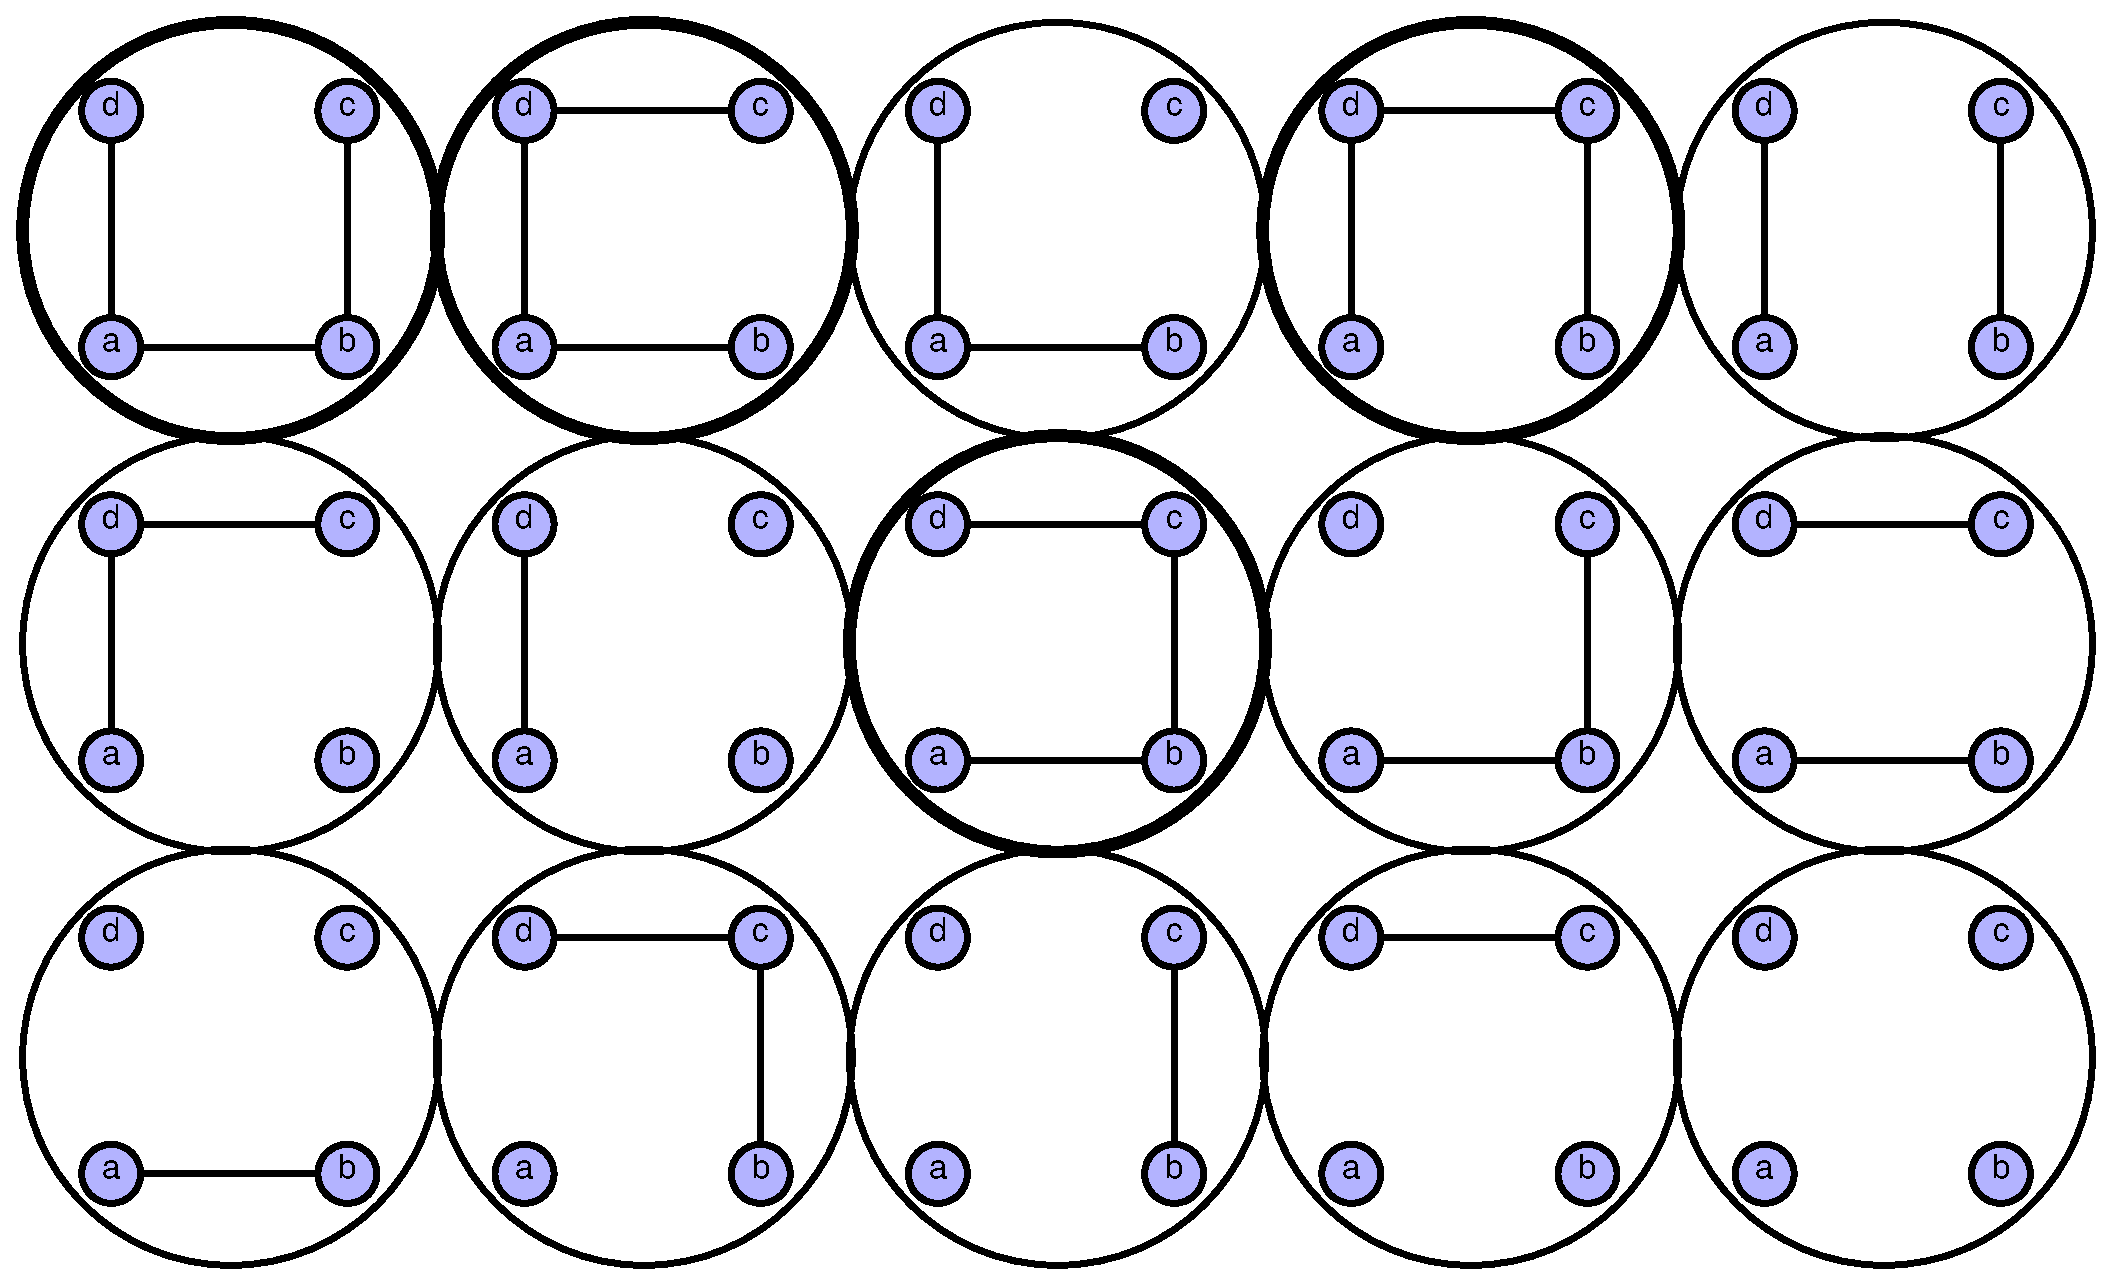
\includegraphics[width=0.9\linewidth]{Images/Matroid}
\caption{graphischer Matroid}
\label{fig:Matroid}
\end{figure}

Die Teilmengen größter Kardinalität sind $M_1:=\{ (a,b),(b,c),(c,d) \},M_2:=\{ (a,b),(b,c),(d,a) \},\\M_3:=\{ (a,b),(c,d),(d,a) \},M_4:=\{ (b,c),(c,d),(d,a) \}$. Es handelt sich dabei um die möglichen Spannbäume des Graphen $G$.
\subsection*{b)}
Es handelt sich um den Algorithmus von Kruskal. Der Algorithmus gibt $B=\{ (a,b),(b,c),(c,d) \}$ aus. Die Abfrage verhindert das Bilden von Zyklen.
\subsection*{c)}
Das Sortieren der Kanten hat im Allgemeinen (also ohne Radix-Sort) eine Laufzeit in $\mathcal{O}(|E| \log |E|)$. Die Schleife läuft über die Menge aller Kanten, also $|E|$ mal. Innerhalb der Schleife gibt es die Abfrage mit der Laufzeit $f(|E|)$ und die Einfüge-Operation, welche mit passender Datenstruktur in konstanter Zeit ausgeführt werden kann. Somit ergibt sich eine Laufzeit in $\mathcal{O}(|E|\log|E|+|E|f(|E|))$.
\subsection*{d)}

\begin{wrapfigure}{l}{0.3\linewidth}
	\centering
	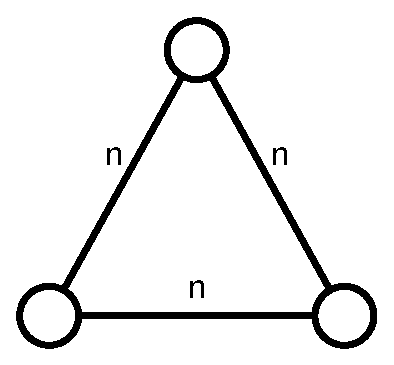
\includegraphics[width=0.5\linewidth]{Images/Beispiel}
	\caption{Sei n eine beliebigen Länge}
	\label{fig:Beispiel}
\end{wrapfigure}
Nein, der Algorithmus ist nicht eindeutig. Man denke sich einen dreieckigen Graphen mit den Kanten $E:=\{ (a,b),(b,c),(c,a) \}$ welche ein einheitliches Kantengewicht aufweisen. Das Ergebnis ist nun vom Sortierverfahren abhängig. So liefern allein stabile und instabile Algorithmen verschiedene Ergebnisse. Mögliche Lösungen wären $L_1:=\{ (a,b),(b,c) \},L_2:=\{ (a,b),(c,a)\},L_3:=\{ (b,c),(c,d) \}$
\end{document}